\namedsubsection{ARM Cortex M0 Processor \label{sec:cortex}}{Pasat}

\todo{Talk about why cortex m0 over m0+}

This section discusses one of the main requirements and one of the essential aspects of the project: using ARM's Cortex M0 processor. This processor is a member of the Cortex-M family and offers a great tradeoff between costs and performance/functionality. It has been designed in order to allow intelligent compromises in terms of power usage, computational power and in the simplicity of the design. It implements a simplified version of the Advanced Microcontroller Bus Architecture (AMBA), the AMBA-Lite Bus, which allows connection to different peripherals. In this way, the Cortex-M0 generally acts as the master device and the peripherals act as slaves. In figure \ref{fig:cortexm0ds}, the schematic for the processor can be seen.\\
\begin{figure}
\centering
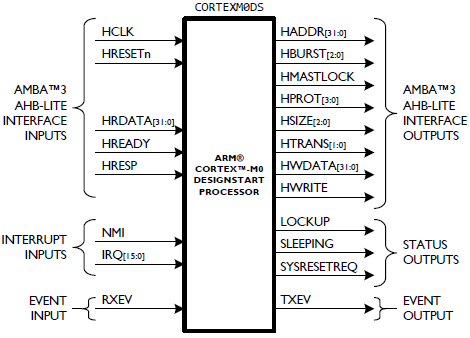
\includegraphics[scale=0.7]{figures/cortexm0ds_schematic.PNG}
\caption{Cortex M0DS schematic \cite{armdesignstart}} \label{fig:cortexm0ds}
\end{figure}
\clearpage

\begin{figure}
\centering
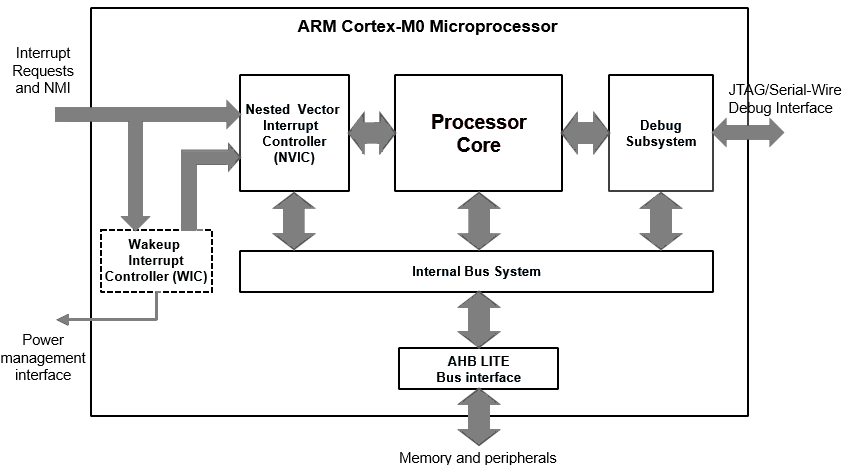
\includegraphics[scale=0.7]{figures/arm_cortexm0_microprocessor.PNG}
\caption{Cortex-M0 Block Diagram \cite{armdesignstart}} \label{fig:cortex_block}
\end{figure}

The Cortex M0 has a 32-bit reduced instruction set computing (RISC) processor. It uses the ARMv6-M(Microcontroller), which is a subset of the ARMv7-M profile but includes fewer instructions. The Cortex M0 is based on a Von-Neumann architecture, having both data and instructions share a single bus interface. It provides a Debug Extension that includes some architectural extensions to support debugging. The ARMv6-M offers support for 56 instructions as a subset of  Thumb-1(16-bit) and Thumb-2(16/32b-bit) which are present in the ARMv6T2. The Cortex M0 block diagram can be seen above in figure \ref{fig:cortex_block}. 

The Cortex M0 has a three-stage pipeline: fetch, decode and exection and includes the 32-bit registers for general and special usages. The Cortex M0+ has only a two-stage pipeline to reduce the power usage.

The Nested Vectored Interrupt Controller (NVIC) handles up to 32 interrupts request signals and one NMI (Non-Maskable Interrupt). It also fulfils tasks such as comparing priorities between  interrupt requests and the current priority level. 

The Debug system handles the program breakpoints, debugging control and the data watchpoints. This can put the processor in a  static state in order for the programmer to evaluate and analyse the status of the processor in that specific moment.

The Wakeup Interrupt Controller (WIC) could be useful for this project because it is used in low-power applications. The microcontroller can be set to enter sleep mode by turning off most of its components. If a interrupt request is sent, this component can inform the unit that handles the power management to power up the system.

\subsubsection{Limitations \label{sec:cortex-limitations}}

Since the sub-threshold Cortex M0+ is such a low-power, lost-cost device, it comes with its limitations. The device only offers 32kB on-chip flash programming memory and 8kB SRAM. Basic applications have been developed for this processor, but in order to allow the implementation of a more complex program, such as exercise recognition, the code and libraries need to be very well optimised. All the unnecessary functionalities available in libraries must be disposed in order to save memory on this constrained system.

One of the major challenges which was encountered in the use of the Cortex M0 is the lack of hardware division or floating point unit. To account for this, there are software libraries which perform these operations however, they can take quite a large number of cycles to perform and hence would be impractical on a constrained system.